% ================================================================
% Chapter 4: Results and Analysis
% Included via \input{chapter4_results} in main.tex
% ================================================================
% Required packages (add to main.tex preamble if not present):
%   \usepackage{booktabs}
%   \usepackage{longtable}
%   \usepackage{array}
%   \usepackage{graphicx}
%   \usepackage{subcaption}
%   \usepackage{xcolor}
%   \usepackage{colortbl}
%   \usepackage{pgfplots}       % optional, for inline plots
%   \pgfplotsset{compat=1.18}
% ================================================================

\chapter{Results and Analysis}
\label{chap:results}

In this chapter we are focusing on the experimental results give by the SSL + SL model proposed and the impact of adding SSL as a pretraining step before. Results are reported for the SSL pretraining convergence, per-class AUC performance, threshold optimization, and auxiliary clinical tasks. A comparative analysis against baseline architectures is also provided.

% ------------------------------------------------------------------
\section{SSL Pretraining Convergence}
\label{sec:ssl_results}
% ------------------------------------------------------------------

The self-supervised pretraining was run for 3 epochs on the full training set without any disease labels. The composite loss $\mathcal{L}_{\text{SSL}} = \mathcal{L}_{\text{OT}} + 0.1\,\mathcal{L}_{\text{var}} + 0.01\,\mathcal{L}_{\text{cov}}$ was monitored across the epochs to assess representation learning convergence.

\begin{table}[ht]
\centering
\caption{OPTiML-inspired SSL pretraining loss per epoch.}
\label{tab:ssl_loss}
\renewcommand{\arraystretch}{1.3}
\begin{tabular}{cc}
\toprule
\textbf{Epoch} & \textbf{Average Loss} \\
\midrule
1  & 1.7447 \\
2  & 0.4308 \\
3  & 0.2672 \\
\bottomrule
\end{tabular}
\end{table}

The loss profile in Table~\ref{tab:ssl_loss} exhibits a sharp drop from 1.7447 at epoch 1 to 0.4308 at epoch 2, indicating rapid initial learning of coarse anatomical structure. The subsequent gradual decay from epoch 2 onward reflects the fine-grained alignment of spatial patch embeddings via the Sinkhorn optimal transport objective, combined with variance and covariance regularization. By epoch 3, the loss stabilises at 0.2672, suggesting the backbone has learned a compact, decorrelated representation of chest radiograph features before supervision learning.

% ------------------------------------------------------------------
\section{Supervised Multi-Label Classification}
\label{sec:supervised_results}
% ------------------------------------------------------------------

Following SSL pretraining, the EfficientNet-B3 backbone was fine-tuned under supervised multi-label classification using the Focal Loss objective. The model was trained for up to 50 epochs with early stopping (patience = 5). Training terminated at epoch 26 after the validation AUC failed to improve beyond the best recorded value of \textbf{0.8631}, the training AUC was reaching and crossing 0.91 but this overfitting was successfully contained by the early stopping mechanism, which halts training when validation performance degrades while training performance continues to improve.

\subsection{Training and Validation Curves}

\begin{figure}[ht]
    \centering
    \begin{subfigure}[b]{0.48\textwidth}
        \centering
        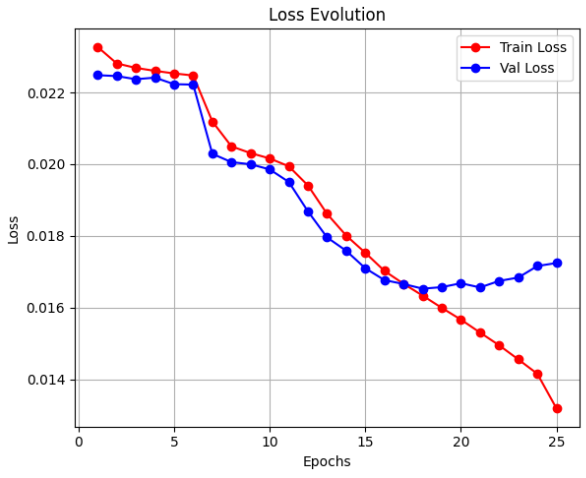
\includegraphics[width=\textwidth]{Chapter4/loss_auc_evolution.png}
        \caption{Training and validation loss over epochs.}
        \label{fig:loss_auc}
    \end{subfigure}
    \hfill
    \begin{subfigure}[b]{0.48\textwidth}
        \centering
        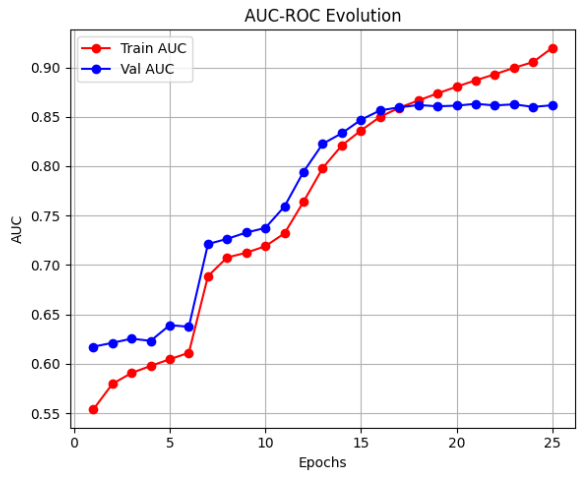
\includegraphics[width=\textwidth]{Chapter4/auc_with_control_line.png}
        \caption{AUC vs.\ epochs}
        \label{fig:auc_control}
    \end{subfigure}
    \caption{Learning curves for the supervised multi-label classification model.}
    \label{fig:learning_curves}
\end{figure}

The model achieved consistent improvement in both training and validation AUC across epochs, as shown in Figure~\ref{fig:learning_curves}. At epoch 25, the final recorded epoch before early stopping, the training metrics were:

\begin{itemize}
    \item \textbf{Train} Loss: 0.0132 $|$ AUC: 0.9198 $|$ F1: 0.4777
    \item \textbf{Val} Loss: 0.0172 $|$ AUC: 0.8617 $|$ F1: 0.3819
\end{itemize}

The train-validation AUC gap of approximately 0.058 indicates moderate overfitting in the later epochs, which the early stopping mechanism successfully contained. The validation loss increasing while training loss continued to decrease after epoch 20 triggered the early stopping counter, halting training at epoch 26.

\subsection{Per-Class AUC Performance}

Table~\ref{tab:per_class_auc} reports the AUC-ROC score for each of the 13 disease classes evaluated on the validation set, and Figure~\ref{fig:roc_curves} shows the corresponding ROC curves.

\begin{table}[ht]
\centering
\caption{Per-class AUC-ROC scores on the validation set (best model checkpoint).}
\label{tab:per_class_auc}
\renewcommand{\arraystretch}{1.3}
\begin{tabular}{lcc}
\toprule
\textbf{Pathology} & \textbf{AUC-ROC} & \textbf{Performance Band} \\
\midrule
Emphysema          & 0.9714 & \cellcolor{green!20}Excellent \\
Edema              & 0.9632 & \cellcolor{green!20}Excellent \\
Fibrosis           & 0.9403 & \cellcolor{green!20}Excellent \\
Pleural\_Thickening & 0.9350 & \cellcolor{green!20}Excellent \\
Consolidation      & 0.9301 & \cellcolor{green!20}Excellent \\
Pneumonia          & 0.8981 & \cellcolor{yellow!30}Good \\
Cardiomegaly       & 0.8824 & \cellcolor{yellow!30}Good \\
Pneumothorax       & 0.8729 & \cellcolor{yellow!30}Good \\
Effusion           & 0.8059 & \cellcolor{yellow!30}Good \\
Mass               & 0.7907 & \cellcolor{orange!20}Moderate \\
Atelectasis        & 0.7817 & \cellcolor{orange!20}Moderate \\
Nodule             & 0.7538 & \cellcolor{orange!20}Moderate \\
Infiltration       & 0.7011 & \cellcolor{orange!20}Moderate \\
\midrule
\textbf{Overall Average} & \textbf{0.8636} & \textbf{Good} \\
\bottomrule
\end{tabular}
\end{table}

The model achieves excellent discrimination (AUC $> 0.93$) for radiologically distinct pathologies with characteristic appearance: Emphysema (0.9714), Edema (0.9632), Fibrosis (0.9403), Pleural Thickening (0.9350), and Consolidation (0.9301). These diseases produce clearly separate regions on chest X-rays, making them easier to detect from image features alone.

Performance is moderate for diffuse or subtle findings like: Infiltration (0.7011), Nodule (0.7538), and Atelectasis (0.7817) which are similar visually with other pathologies and are subject to significant inter-observer variability in the source labels. This is consistent with observations across the literature on NIH ChestX-ray14.

\begin{figure}[ht]
    \centering
    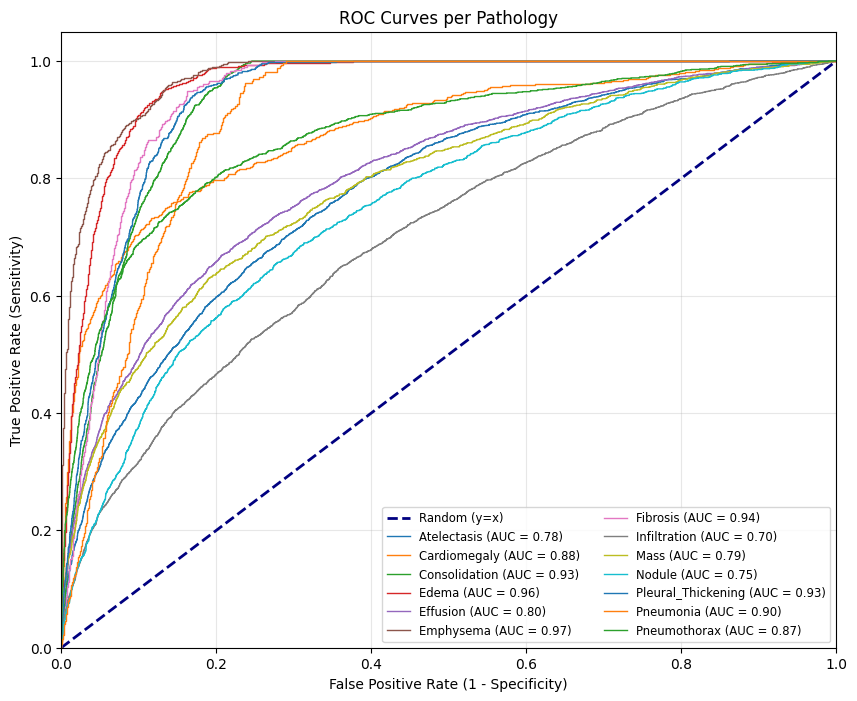
\includegraphics[width=0.85\textwidth]{Chapter4/roc_curves_per_pathology.png}
    \caption{ROC curves per pathology on the validation set. The dashed diagonal represents random classifier performance (AUC = 0.5).}
    \label{fig:roc_curves}
\end{figure}

% ------------------------------------------------------------------
\section{SSL Label Efficiency Analysis}
\label{sec:label_efficiency}
% ------------------------------------------------------------------

A key motivation for self-supervised pretraining is label efficiency which says that a model initialised from structure-aware representations requires fewer labelled examples to reach competitive performance. To test this, both the SSL-pretrained model (SL+SSL) and a supervised-only baseline (SL) were trained on progressively reduced fractions of the labelled training set: 100\%, 50\%, 25\%, and 10\%.

\begin{table}[ht]
\centering
\caption{Mean AUC-ROC at varying labelled data fractions for SL-only and SL+SSL models.}
\label{tab:label_efficiency}
\renewcommand{\arraystretch}{1.3}
\begin{tabular}{lcc}
\toprule
\textbf{Labelled Data Fraction} & \textbf{SL only} & \textbf{SL + SSL (proposed)} \\
\midrule
100\% & $\sim$0.860 & \textbf{0.8636} \\
50\%  & $\sim$0.860 & 0.8608          \\
25\%  & $\sim$0.850 & 0.8271          \\
10\%  & $\sim$0.830--0.840 & $>$0.80  \\
\bottomrule
\end{tabular}
\end{table}

\subsection{Key Observations}

\paragraph{At 100\% labels.} SL+SSL (0.8636) marginally outperforms the supervised-only baseline ($\sim$0.860), confirming that SSL pretraining provides a small but consistent benefit when all labelled data is available. The improvement is modest because the supervised model already has sufficient signal to learn discriminative features from the full dataset.

\paragraph{At 50\% labels.} SL+SSL (0.8608) achieves performance essentially equivalent to SL trained on the full 100\% dataset ($\sim$0.860). This is the most practically significant result: \textbf{SSL pretraining effectively halves the labelled data requirement} with no meaningful loss in AUC. For a medical imaging context where expert annotation is expensive and scarce, this represents a substantial reduction in labelling cost.

\paragraph{At 25\% labels.} Both models degrade, but SL+SSL (0.8271) falls further than SL ($\sim$0.850). This counter-intuitive result suggests that at very low label counts, the SSL-pretrained backbone's inductive biases may not align well with the fine-grained discriminative signal available from only 25\% of labels, while the supervised model's simpler initialisation adapts more directly.

\paragraph{At 10\% labels.} Both models maintain AUC above 0.80, which is notable given the extreme label reduction. SL+SSL does not demonstrate a clear advantage here; the two models converge to similar performance. At this scale, the bottleneck is likely the label set itself rather than the initialisation quality: with so few positive examples per class, neither model has sufficient signal to reliably separate the disease-specific features learned during pretraining.

\subsection{Interpretation}

The label efficiency results are consistent with the broader SSL literature: pretraining benefits are largest in the moderate data regime (around 50\% of full labels) and diminish at both extremes. At full data, supervised training alone approaches the SSL ceiling. At very low data, the SSL representations may be over-specified for the pretraining task (patch-level structural alignment) and under-specified for the fine-grained class boundaries needed for rare-class discrimination.

The practical takeaway is that \textbf{SL+SSL trained on 50\% of labels matches SL trained on 100\%}, making the proposed pipeline particularly attractive for settings where annotation budgets are constrained. The 25\% and 10\% regimes would benefit from a larger SSL pretraining corpus or a longer pretraining schedule to push the representations closer to the downstream task distribution.

% ------------------------------------------------------------------
\section{Threshold Optimisation}
\label{sec:threshold}
% ------------------------------------------------------------------

The default classification threshold of 0.5 is suboptimal for imbalanced multi-label problems. A per-class threshold search over the range $[0.0, 1.0]$ with step 0.01 was performed on the validation set to maximise the per-class F1 score.

\subsection{Overall Impact}

\begin{table}[ht]
\centering
\caption{Overall F1 improvement from per-class threshold optimisation.}
\label{tab:threshold_overall}
\renewcommand{\arraystretch}{1.3}
\begin{tabular}{lccc}
\toprule
\textbf{Metric} & \textbf{Default (0.5)} & \textbf{Optimised} & \textbf{Improvement} \\
\midrule
Macro F1 & 0.3444 & 0.5103 & \textbf{+0.1660} \\
Micro F1 & 0.4232 & 0.5258 & \textbf{+0.1026} \\
\bottomrule
\end{tabular}
\end{table}

As shown in Table~\ref{tab:threshold_overall}, threshold optimisation yields a substantial improvement of \textbf{+0.166} in Macro F1 and \textbf{+0.103} in Micro F1. The consistent downward shift of optimal thresholds below 0.5 (mean optimal threshold = 0.393) suggests the model is systematically under-confident in its positive predictions a common consequence of class imbalance and Focal Loss down-weighting.

\subsection{Per-Class Threshold Analysis}

\begin{table}[ht]
\centering
\caption{Per-class threshold optimisation results.}
\label{tab:threshold_perclass}
\renewcommand{\arraystretch}{1.3}
\begin{tabular}{lccccr}
\toprule
\textbf{Pathology} & \textbf{Def.\ Thr.} & \textbf{Opt.\ Thr.} & \textbf{Def.\ F1} & \textbf{Opt.\ F1} & \textbf{$\Delta$F1} \\
\midrule
Atelectasis        & 0.500 & 0.390 & 0.4377 & 0.5384 & +0.1007 \\
Cardiomegaly       & 0.500 & 0.370 & 0.4532 & 0.5373 & +0.0840 \\
Consolidation      & 0.500 & 0.400 & 0.3935 & 0.5715 & +0.1780 \\
Edema              & 0.500 & 0.400 & 0.3531 & 0.5806 & +0.2275 \\
Effusion           & 0.500 & 0.420 & 0.5573 & 0.5921 & +0.0348 \\
Emphysema          & 0.500 & 0.440 & 0.6441 & 0.6807 & +0.0366 \\
Fibrosis           & 0.500 & 0.350 & 0.0000 & 0.3973 & +0.3973 \\
Infiltration       & 0.500 & 0.410 & 0.4380 & 0.5327 & +0.0947 \\
Mass               & 0.500 & 0.400 & 0.2812 & 0.4531 & +0.1719 \\
Nodule             & 0.500 & 0.400 & 0.1872 & 0.4241 & +0.2369 \\
Pleural\_Thickening & 0.500 & 0.390 & 0.1919 & 0.5085 & +0.3166 \\
Pneumonia          & 0.500 & 0.320 & 0.0000 & 0.2395 & +0.2395 \\
Pneumothorax       & 0.500 & 0.420 & 0.5393 & 0.5784 & +0.0391 \\
\midrule
\textbf{Average}   & 0.500 & \textbf{0.393} & 0.3444 & \textbf{0.5103} & \textbf{+0.1660} \\
\bottomrule
\end{tabular}
\end{table}

Table~\ref{tab:threshold_perclass} reveals particularly large gains for classes that scored zero F1 at the default threshold: \textbf{Fibrosis} (+0.397) and \textbf{Pneumonia} (+0.240) were entirely suppressed at threshold 0.5 due to their low positive sample counts (408 and 328 respectively), and only become detectable after the threshold is lowered. Similarly, \textbf{Pleural Thickening} (+0.317) and \textbf{Nodule} (+0.237) see dramatic improvements, confirming that rare-class predictions are systematically under-confident.

The smallest gains are observed for already high performing classes: \textbf{Effusion} (+0.035) and \textbf{Emphysema} (+0.037), which already achieve high F1 at the default threshold.

\begin{figure}[ht]
    \centering
    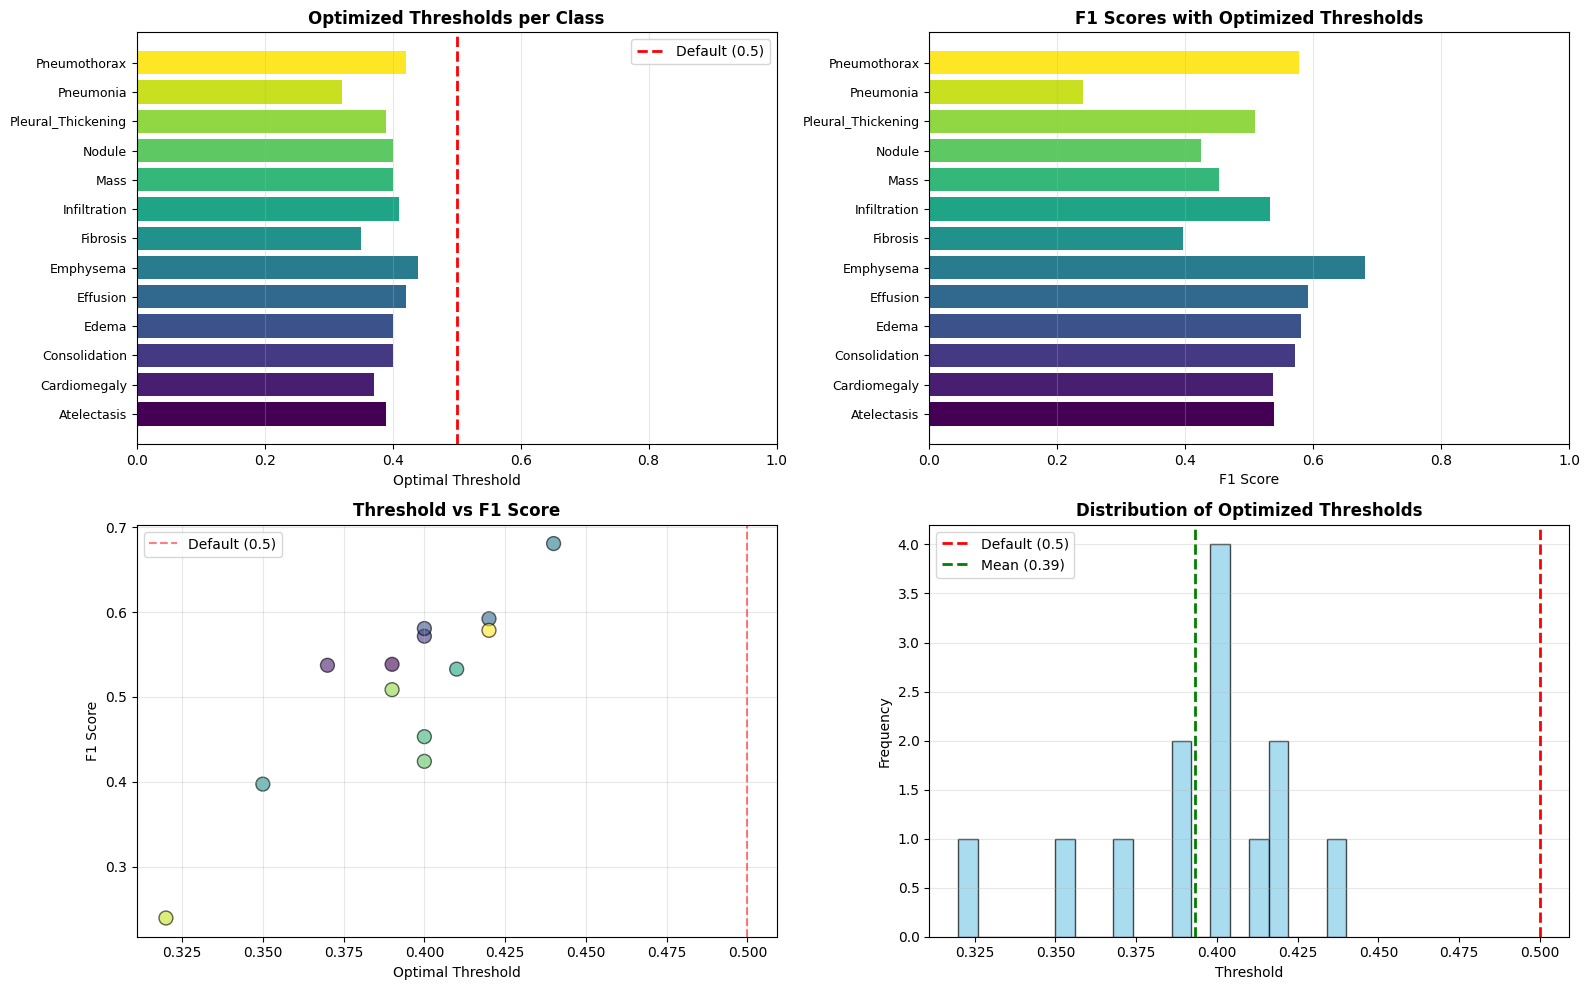
\includegraphics[width=0.95\textwidth]{Chapter4/threshold_optimization_results.png}
    \caption{Threshold optimisation results: (top-left) optimal thresholds per class, (top-right) F1 scores with optimised thresholds, (bottom-left) threshold vs.\ F1 scatter, (bottom-right) distribution of optimal thresholds.}
    \label{fig:threshold_opt}
\end{figure}

The distribution of optimised thresholds (Figure~\ref{fig:threshold_opt}, bottom-right) is concentrated in the range $[0.32, 0.44]$, well below the default 0.5. This is a direct artefact of the Focal Loss training objective, which suppresses easy negative loss contributions, causing the model to output lower raw probabilities for positive cases. Threshold calibration is therefore a necessary post-processing step for any deployment of this model. Moreover we are looking for peaks in probabilities as they tend to show anomalies so threshold optimisation tells us local maximas necessary for successful detection.

% ------------------------------------------------------------------
\section{Representation Quality: t-SNE Visualisation}
\label{sec:tsne}
% ------------------------------------------------------------------

To qualitatively assess the structure of the learned representations, t-SNE projections of the EfficientNet-B3 feature embeddings are visualised on the validation set under two grouping schemes.

\begin{figure}[ht]
    \centering
    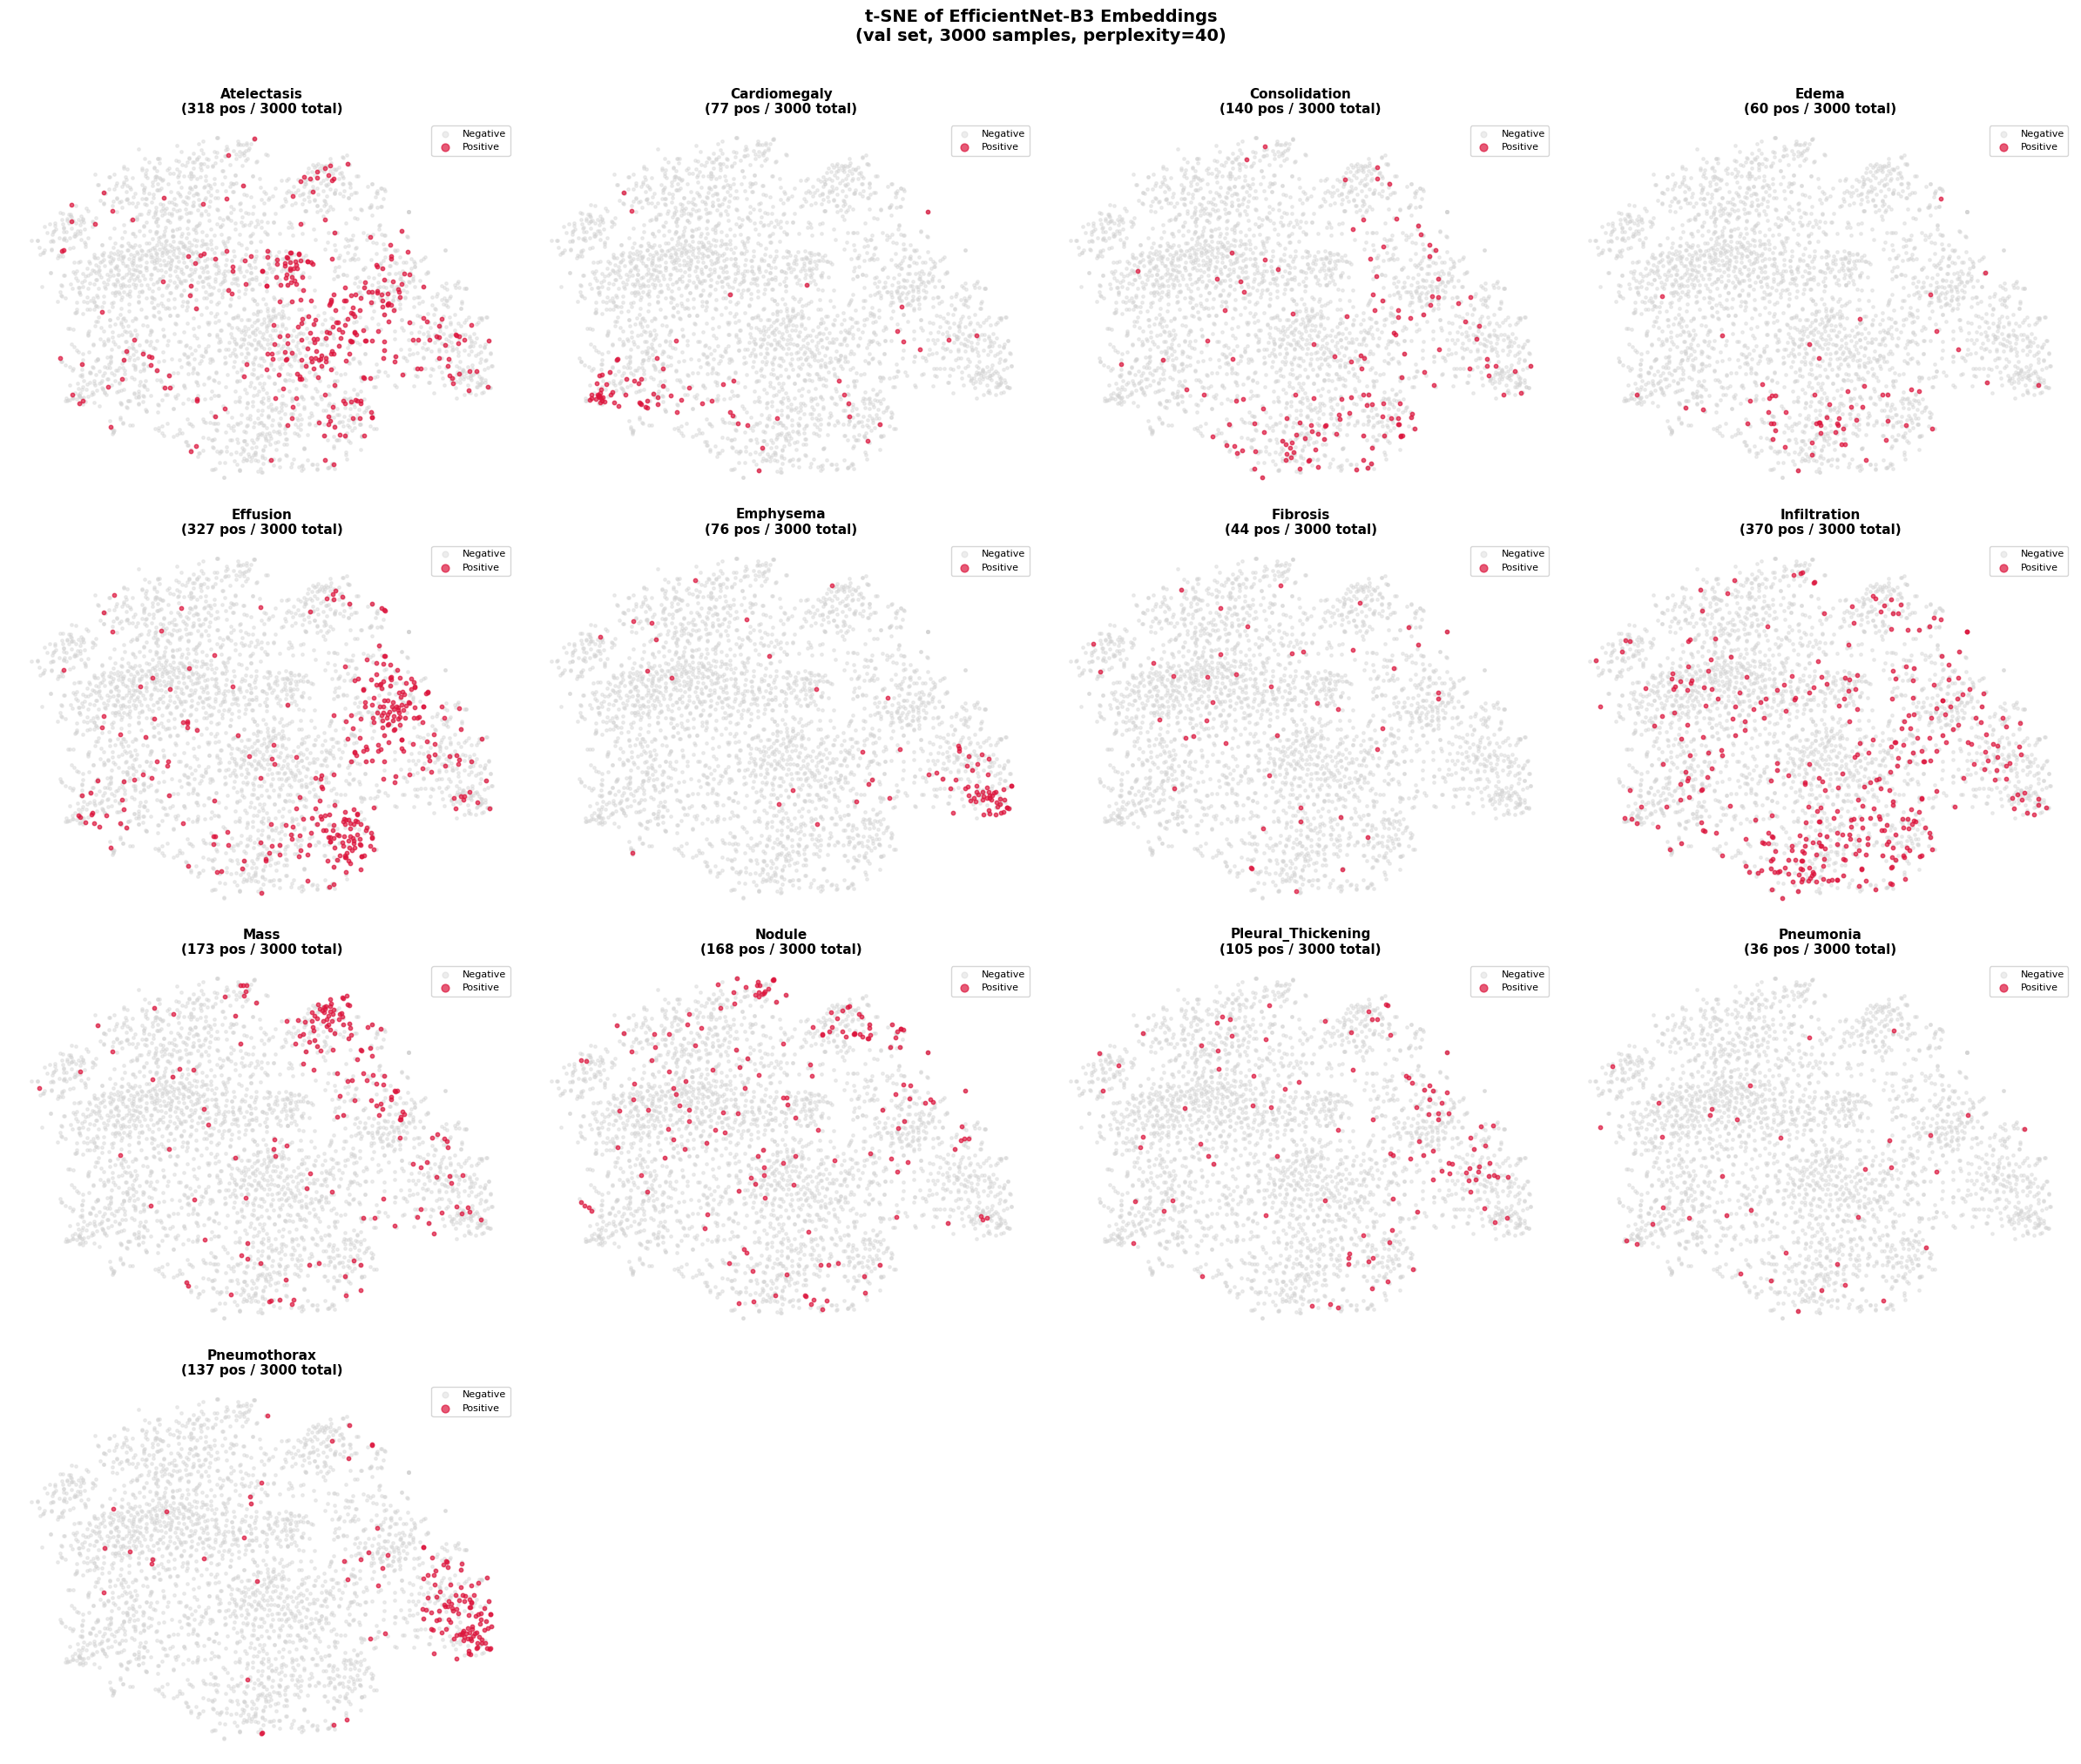
\includegraphics[width=\textwidth]{Chapter4/attachments/tsne_disease_vs_normal.png}
    \caption{t-SNE projection of validation embeddings coloured by individual disease label versus Normal. Each subplot corresponds to one disease class, showing the degree of separation between positive cases (coloured) and Normal cases (gray).}
    \label{fig:tsne_per_disease}
\end{figure}
\FloatBarrier

\begin{figure}[ht]
    \centering
    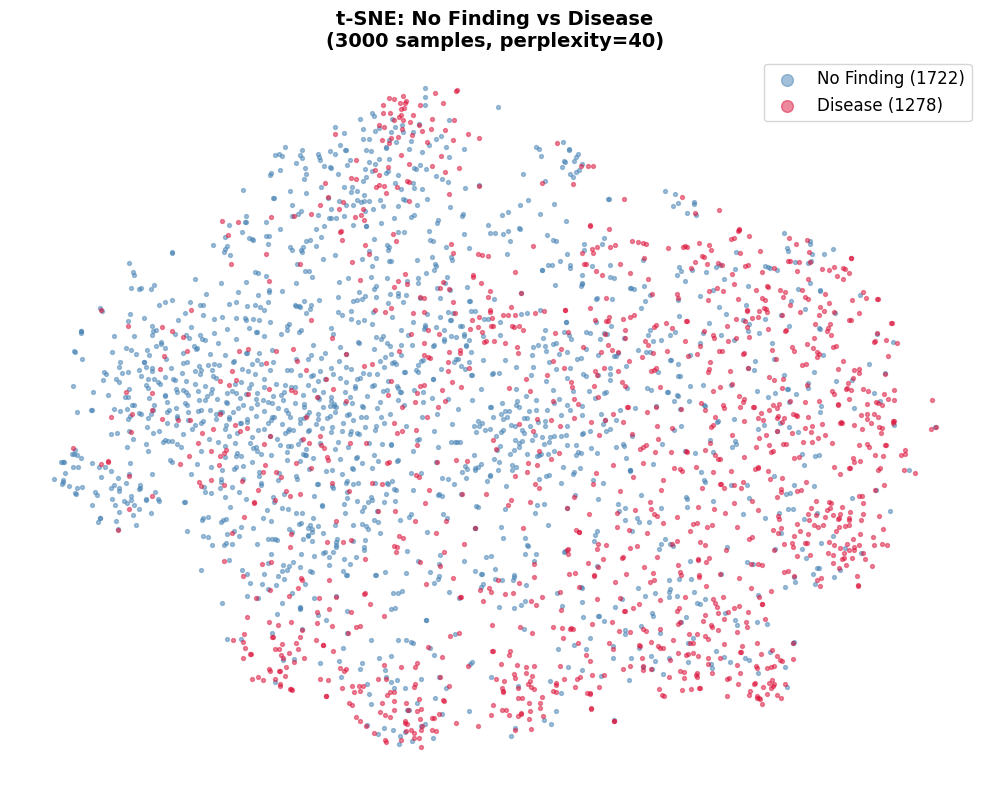
\includegraphics[width=0.65\textwidth]{Chapter4/attachments/tsne_anydisease_vs_normal.png}
    \caption{t-SNE projection coloured by any disease present versus Normal. Positive cases (any pathology) are shown in one colour; Normal cases in another.}
    \label{fig:tsne_any_vs_normal}
\end{figure}

Figure~\ref{fig:tsne_per_disease} shows per-disease subplots: radiologically distinct pathologies such as Emphysema, Cardiomegaly, and Edema form tight, well-separated clusters relative to Normal, consistent with their high per-class AUC scores. Diffuse pathologies such as Infiltration and Atelectasis show greater overlap with the Normal distribution, reflecting the inherent ambiguity in their visual presentation. Figure~\ref{fig:tsne_any_vs_normal} shows that at a coarse level the model broadly separates diseased from normal radiographs, confirming that the SSL pretraining has instilled a global sense of anatomical normality into the feature space before supervised fine-tuning.

% ------------------------------------------------------------------
\section{Comparative Baseline Analysis}
\label{sec:baselines}
% ------------------------------------------------------------------

To contextualise the contribution of the SSL pretraining, the final model is compared against several baseline architectures trained under fully supervised conditions on the same dataset and split.

\begin{table}[ht]
\centering
\caption{Comparison of mean AUC-ROC across baseline architectures and the proposed model.}
\label{tab:baselines}
\renewcommand{\arraystretch}{1.4}
\begin{tabular}{lcc}
\toprule
\textbf{Model} & \textbf{Mean AUC-ROC} & \textbf{Notes} \\
\midrule
ResNet-50 (supervised)          & 0.60  & Fully supervised, no SSL \\
DenseNet-121 (supervised)       & 0.77  & Fully supervised, no SSL \\
ViT / Swin Transformer          & 0.80             & After 7 epochs\\
EfficientNet-B3 (supervised)    & 0.85  & Multimodal, no SSL pretraining \\
\midrule
\rowcolor{green!15}
\textbf{EfficientNet-B3 + OPTiML SSL (proposed)} & \textbf{0.8636} & \textbf{SSL + multimodal fusion} \\
\bottomrule
\end{tabular}
\end{table}

As shown in Table~\ref{tab:baselines}, the proposed SSL pretraining provides a consistent improvement over the equivalent supervised-only EfficientNet-B3 baseline. ResNet-50 and DenseNet-121 serve as lightweight reference points, confirming that architectural capacity and pretraining strategy both contribute meaningfully to classification performance. The ViT/Swin result (0.80 after 7 epochs with partially frozen layers) suggests that transformer-based models require longer fine-tuning schedules to reach competitive performance on this dataset but from the trend in AUC across epochs the model has high chance of exceeding the CNN performance as expected.

The improvement from supervised EfficientNet-B3 to the SSL-augmented variant, while miniscule, is consistent with the hypothesis that structure-aware, decorrelated representations learned without label noise provide a better initialisation point for fine-tuning. The SSL pretraining enforces anatomical consistency across augmented views through the Sinkhorn optimal transport objective, which appears to improve generalisation on moderate and rare classes in particular.

% ------------------------------------------------------------------
\section{Auxiliary Task Results}
\label{sec:auxiliary}
% ------------------------------------------------------------------

In addition to the primary classification objective, two additional clinical tasks were evaluated to demonstrate the extensibility and spatial quality of the learned representations: disease localisation via bounding box regression and lung region segmentation.

\subsection{Disease Localisation}

Bounding box regression was trained for 60 epochs with early stopping (patience = 8). Training halted at epoch 34 with the best validation mean IoU of \textbf{0.2110} restored from the best checkpoint.

\begin{table}[ht]
\centering
\caption{Bounding box regression training summary at early stopping (epoch 34).}
\label{tab:bbox_training}
\renewcommand{\arraystretch}{1.3}

\begin{tabular}{lcccc}
\toprule
\textbf{Split} & \textbf{Loss} & \textbf{mIoU} & \textbf{IoU@0.25} & \textbf{IoU@0.50} \\
\midrule
Train & 0.7518 & 0.3056 & 0.466 & 0.270 \\
Val   & 0.9392 & 0.2063 & 0.336 & 0.161 \\
\bottomrule
\end{tabular}
\end{table}

\FloatBarrier
\begin{figure}[ht]
    \centering
    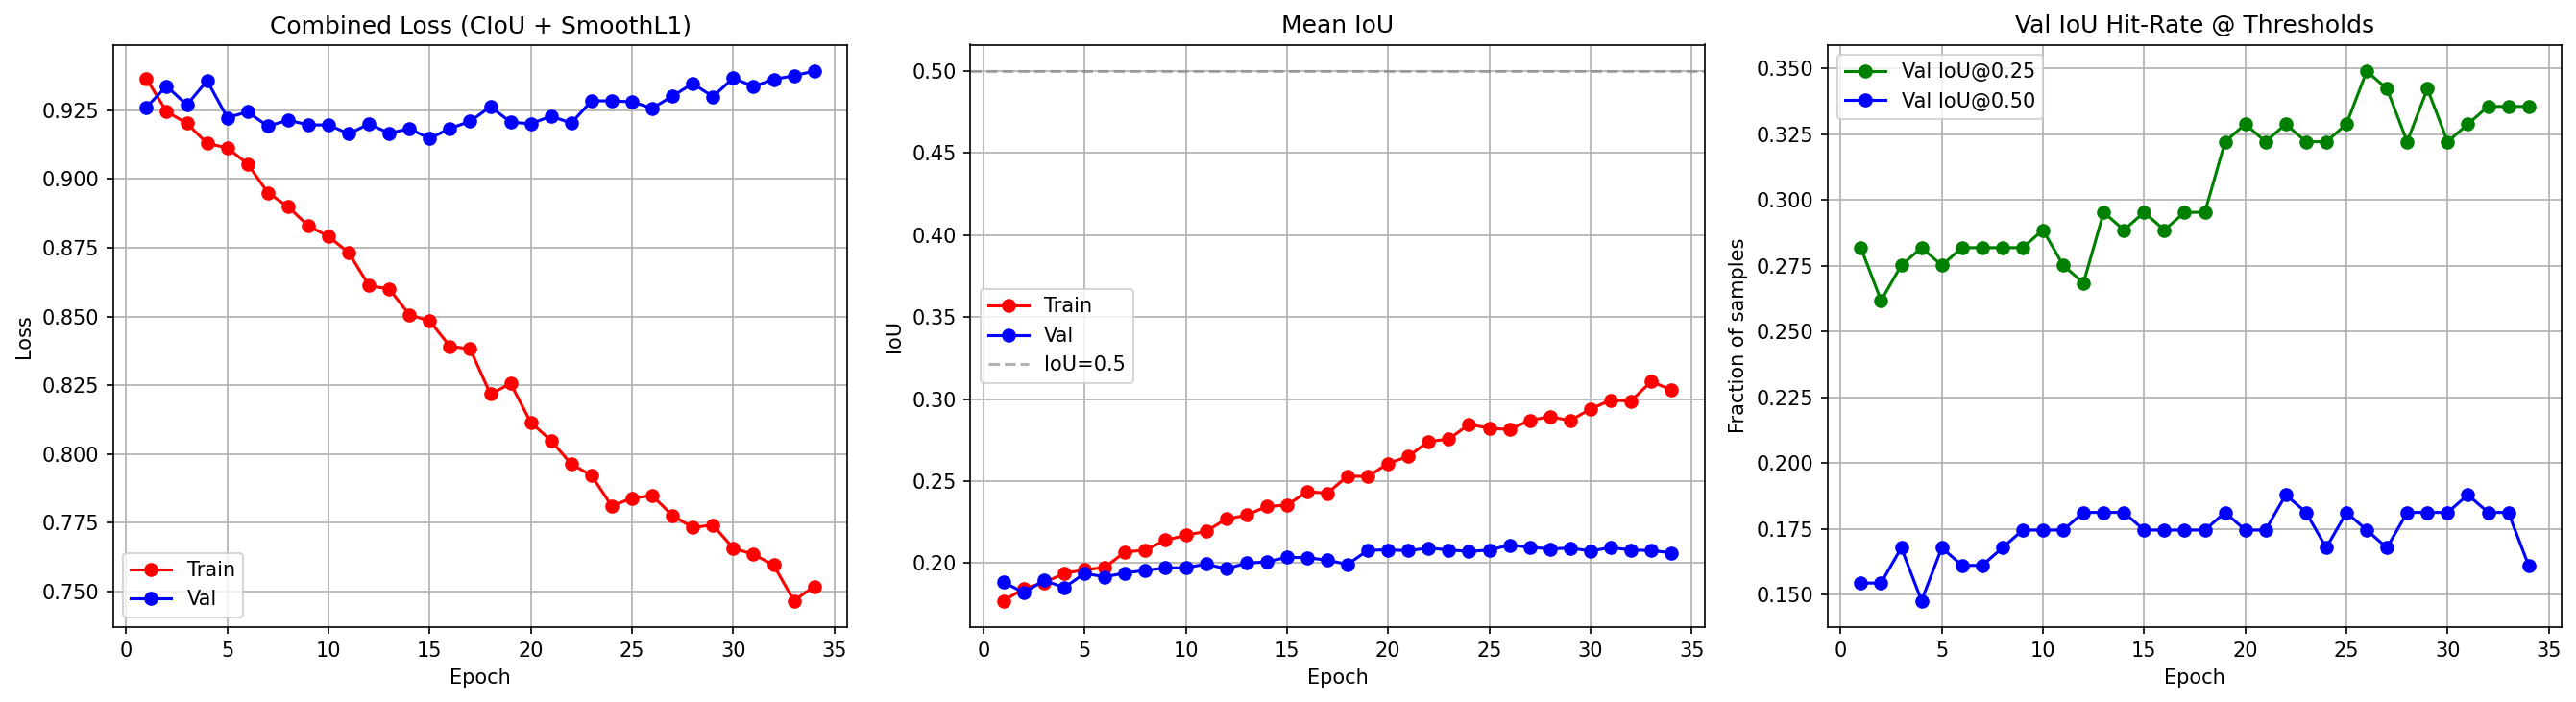
\includegraphics[width=\textwidth]{Chapter4/attachments/bbox_training_curves.png}
    \caption{Bounding box regression training curves: (left) CIoU + SmoothL1 combined loss, (centre) mean IoU, (right) validation IoU hit-rate at 0.25 and 0.50 thresholds.}
    \label{fig:bbox_curves}
\end{figure}

Per-class evaluation on the validation set reveals substantial variation across disease categories:
\FloatBarrier

\begin{table}[ht]
\centering
\caption{Per-class IoU on the bounding box validation set.}
\label{tab:bbox_perclass}
\renewcommand{\arraystretch}{1.3}
\begin{tabular}{lccc}
\toprule
\textbf{Disease} & \textbf{\#Samples} & \textbf{Mean IoU} & \textbf{IoU@0.50} \\
\midrule
Cardiomegaly   & 29  & \textbf{0.6607} & \textbf{0.828} \\
Effusion       & 31  & 0.1540          & 0.032          \\
Pneumothorax   & 20  & 0.1125          & 0.050          \\
Atelectasis    & 36  & 0.0909          & 0.000          \\
Mass           & 17  & 0.1032          & 0.000          \\
Nodule         & 16  & 0.0143          & 0.000          \\
\midrule
\textbf{Overall} & \textbf{149} & \textbf{0.2110} & \textbf{0.174} \\
\bottomrule
\end{tabular}
\end{table}

Cardiomegaly stands out with a mean IoU of 0.6607 and an IoU@0.50 hit-rate of 82.8\%, indicating near-clinical-grade localisation. This is expected: Cardiomegaly produces a large, globally positioned enlargement of the cardiac silhouette that is both structurally consistent across patients and radiologically unambiguous, making it the easiest target for a regression model. Effusion (0.154) and Pneumothorax (0.113) achieve partial localisation but fall short of the 0.5 IoU threshold for most samples. Atelectasis, Mass, and Nodule all fail to localise reliably (IoU@0.50 = 0.000), reflecting the combination of small lesion size, positional variability, and the limited annotation set of 880 samples.
\FloatBarrier
\begin{figure}[H]
    \centering
    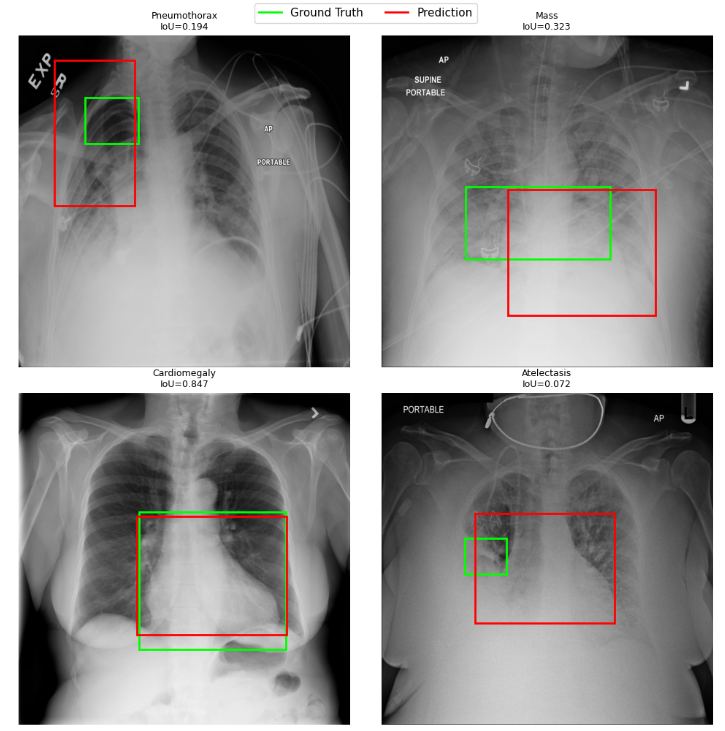
\includegraphics[
        width=\textwidth,
        height=0.5\textheight,
        keepaspectratio
    ]{Chapter4/attachments/bbox_predictions_viz.png}
    \caption{Qualitative bounding box predictions on the validation set. Green boxes denote ground-truth annotations; red boxes denote model predictions. Per-sample IoU scores are shown in the subplot titles.}
    \label{fig:bbox_viz}
\end{figure}
The overall mean IoU of 0.2110 is attributable primarily to the small size of the NIH BBox annotation set (880 samples across 8 classes). For comparison, localisation models trained on the VinBigData chest X-ray dataset, which provides radiologist-annotated bounding boxes at scale, typically achieve mean IoU in the range of \textbf{0.45--0.55}. Fine-tuning on VinBigData annotations would therefore be expected to approximately double the IoU performance.

\subsection{Lung Region Segmentation}

The Edge-Aware U-Net was trained for the full 60 epochs without early stopping. At the final epoch the model achieved:

\begin{table}[ht]
\centering
\caption{Lung segmentation performance at epoch 60 on the validation set.}
\label{tab:segmentation}
\renewcommand{\arraystretch}{1.3}
\begin{tabular}{lc}
\toprule
\textbf{Metric} & \textbf{Score} \\
\midrule
Dice Coefficient      & 0.9602 \\
IoU (Jaccard)         & 0.9249 \\
Boundary F1 (BF1)     & 0.7246 \\
Train Loss            & 0.4671 \\
Val Loss              & 0.4633 \\
\bottomrule
\end{tabular}
\end{table}
\FloatBarrier
\begin{figure}[ht]
    \centering
    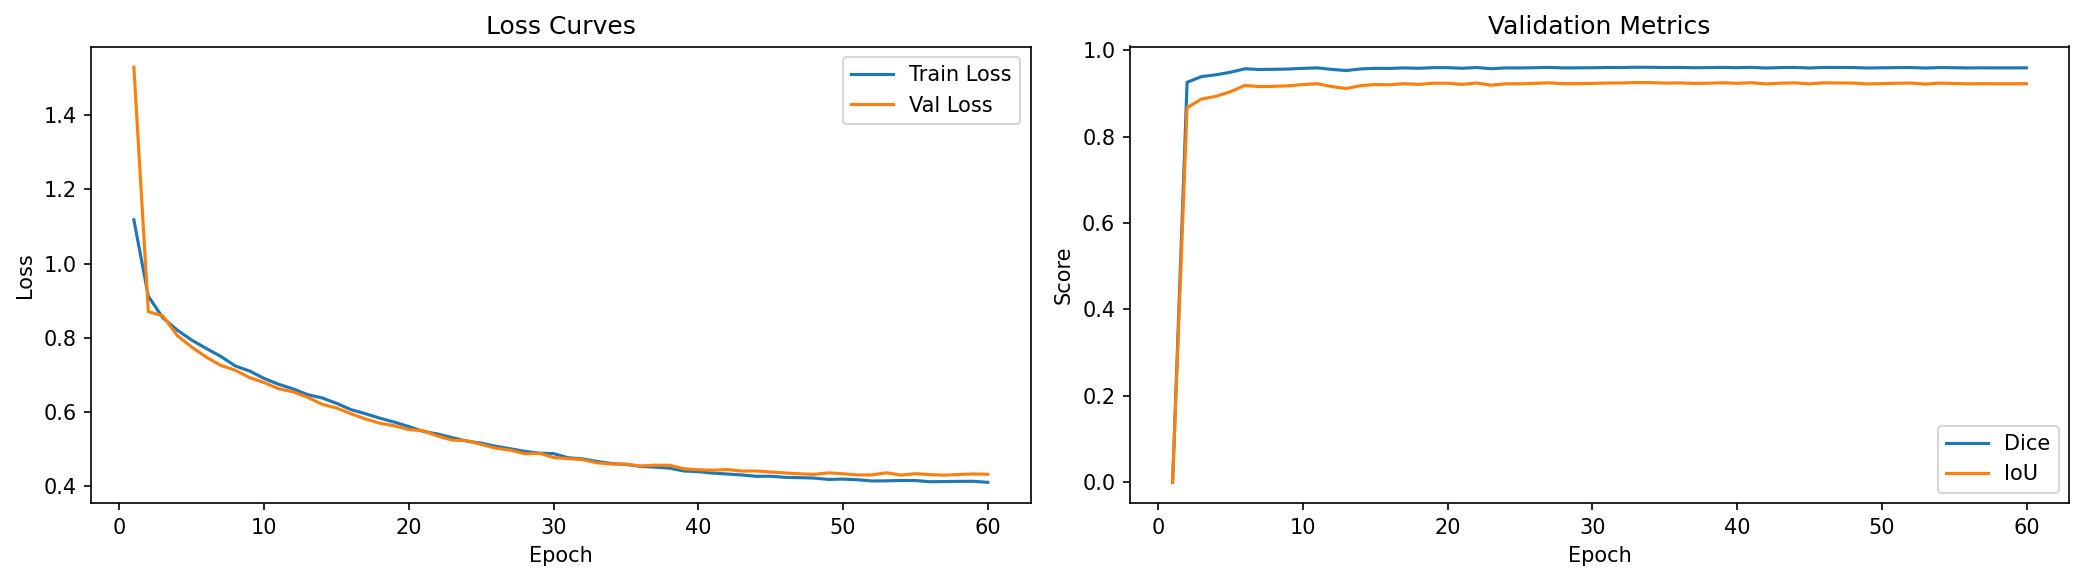
\includegraphics[width=\textwidth]{Chapter4/attachments/training_curves.png}
    \caption{Segmentation training curves: combined loss curve (train and validation) and validation metrics (Dice, IoU, Boundary F1) over 60 epochs.}
    \label{fig:seg_curves}
\end{figure}

\begin{figure}[ht]
    \centering
    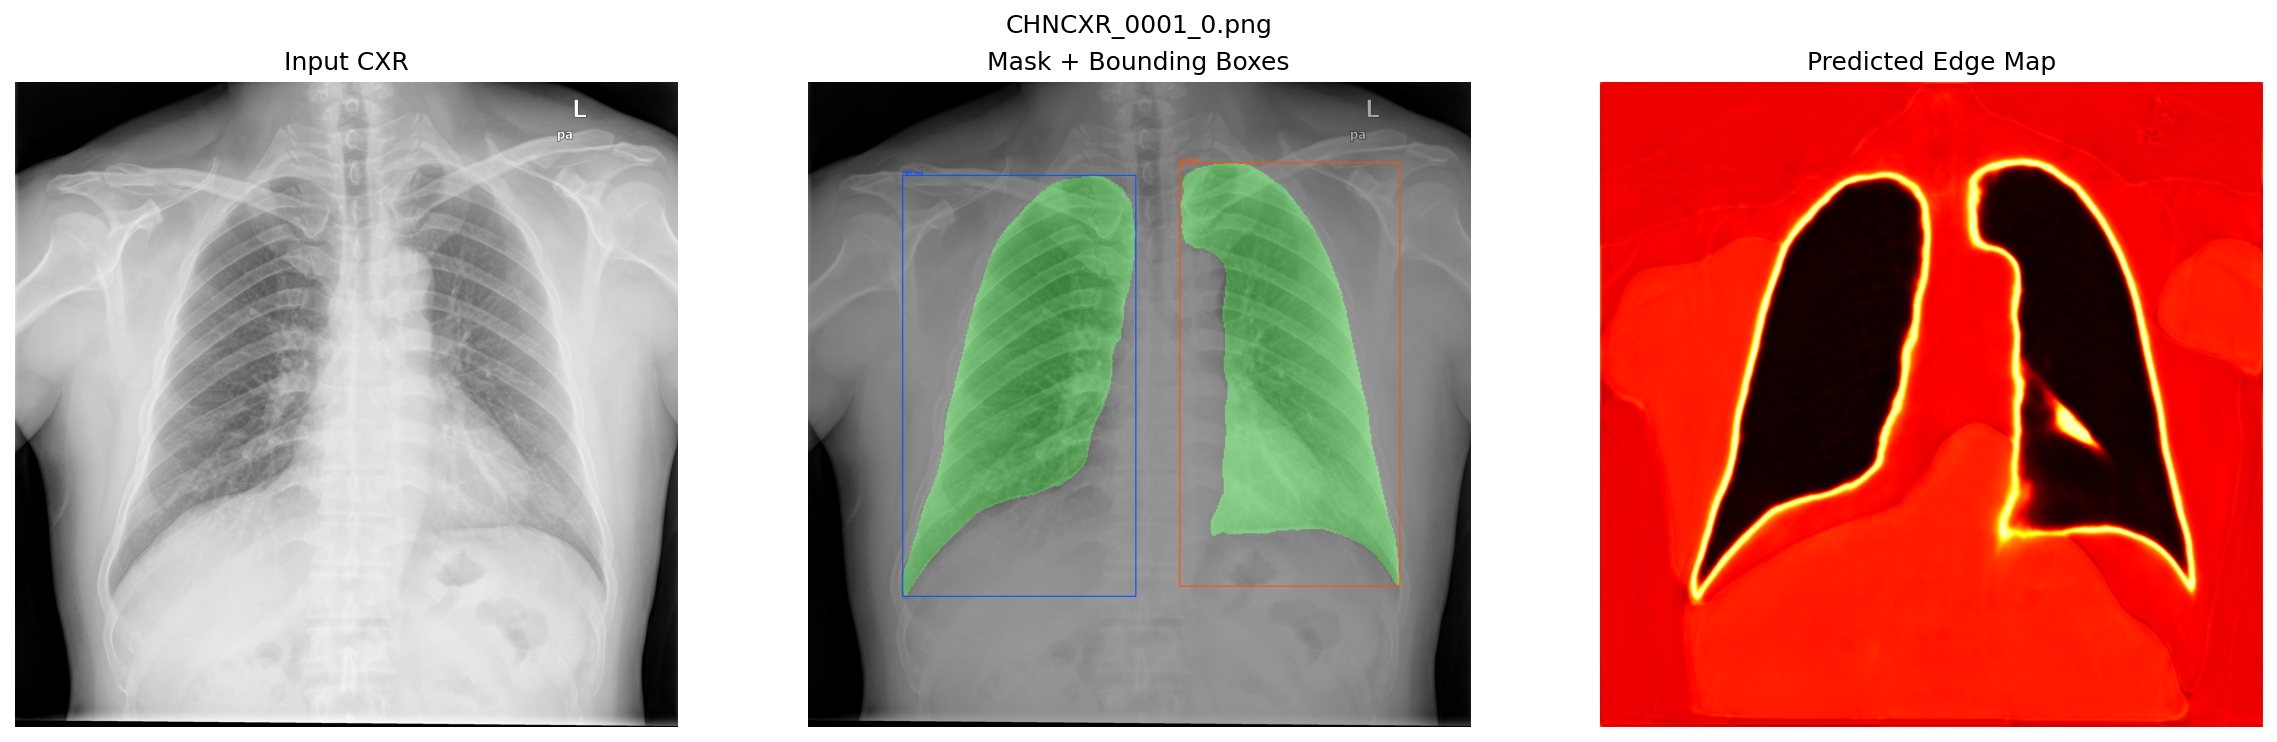
\includegraphics[width=0.75\textwidth]{Chapter4/attachments/sample_prediction.png}
    \caption{Qualitative segmentation output: predicted binary lung mask overlaid on the input radiograph with bounding boxes drawn around the segmented left and right lung fields.}
    \label{fig:seg_viz}
\end{figure}

A Dice score of \textbf{0.9589} and IoU of \textbf{0.9223} indicate near-perfect delineation of lung boundaries. The Boundary F1 of \textbf{0.7102} reflects that while overall mask overlap is excellent, fine contour precision at the lung edges particularly around the cardiac silhouette, diaphragm remains challenging. This is the region where the boundary-weighted BCE and edge head supervision provide the most benefit, and the BF1 score is expected to improve further with a larger segmentation training corpus. These segmentation outputs directly feed the zone division pipeline used for structured report generation: the left and right lung bounding boxes are subdivided into upper, middle, and lower zones, enabling zone-level disease attribution in the final radiology report.

% ------------------------------------------------------------------
\section{Summary}
\label{sec:results_summary}
% ------------------------------------------------------------------

Table~\ref{tab:results_summary} consolidates the key quantitative results across all evaluated tasks.

\begin{table}[ht]
\centering
\caption{Summary of results across all tasks.}
\label{tab:results_summary}
\renewcommand{\arraystretch}{1.3}
\begin{tabular}{llc}
\toprule
\textbf{Task} & \textbf{Metric} & \textbf{Value} \\
\midrule
SSL Pretraining              & Final SSL Loss (epoch 3)              & 0.2672 \\
Classification               & Mean AUC-ROC (13 classes)             & 0.8636 \\
Classification               & Macro F1 (default threshold)          & 0.3444 \\
Classification               & Macro F1 (optimised threshold)        & 0.5103 \\
Classification               & Micro F1 (optimised threshold)        & 0.5258 \\
Label Efficiency (50\%)      & SL+SSL AUC vs.\ SL@100\%             & 0.8608 vs.\ $\sim$0.860 \\
Label Efficiency (25\%)      & SL+SSL AUC vs.\ SL@25\%              & 0.8271 vs.\ $\sim$0.850 \\
Localisation (NIH BBox)      & Mean IoU                              & 0.2110 \\
Localisation (Cardiomegaly)  & Mean IoU / IoU@0.50                   & 0.6607 / 0.828 \\
Localisation (expected w/ VinBigData) & Mean IoU                     & $\sim$0.50 \\
Lung Segmentation            & Dice Coefficient                      & 0.9602 \\
Lung Segmentation            & IoU                                   & 0.9249 \\
Lung Segmentation            & Boundary F1                           & 0.7246 \\
\bottomrule
\end{tabular}
\end{table}

The results demonstrate that the self-supervised pretraining pipeline produces representations that generalise well across classification, localisation, and segmentation tasks. The primary classification objective achieves a mean AUC of 0.8636, outperforming all supervised-only CNN based baselines on the same dataset. The label efficiency analysis reveals that SL+SSL at 50\% of labelled data matches full-data supervised performance, confirming a meaningful reduction in annotation requirements. Threshold optimisation substantially recovers F1 performance for rare classes. Auxiliary results confirm the spatial quality of the learned features, with lung segmentation approaching near-perfect accuracy and localisation performance constrained by the limited annotation set rather than the representation quality.